\documentclass[14pt]{extbook}
\usepackage{multicol, enumerate, enumitem, hyperref, color, soul, setspace, parskip, fancyhdr} %General Packages
\usepackage{amssymb, amsthm, amsmath, latexsym, units, mathtools} %Math Packages
\everymath{\displaystyle} %All math in Display Style
% Packages with additional options
\usepackage[headsep=0.5cm,headheight=12pt, left=1 in,right= 1 in,top= 1 in,bottom= 1 in]{geometry}
\usepackage[usenames,dvipsnames]{xcolor}
\usepackage{dashrule}  % Package to use the command below to create lines between items
\newcommand{\litem}[1]{\item#1\hspace*{-1cm}\rule{\textwidth}{0.4pt}}
\pagestyle{fancy}
\lhead{Progress Quiz 6}
\chead{}
\rhead{Version B}
\lfoot{4563-7456}
\cfoot{}
\rfoot{Summer C 2021}
\begin{document}

\begin{enumerate}
\litem{
First, find the equation of the line containing the two points below. Then, write the equation in the form $ y=mx+b $ and choose the intervals that contain $m$ and $b$.\[ (6, 6) \text{ and } (9, 11) \]\begin{enumerate}[label=\Alph*.]
\item \( m \in [-7.67, 0.33] \hspace*{3mm} b \in [25.8, 29.2] \)
\item \( m \in [-0.33, 8.67] \hspace*{3mm} b \in [3.7, 5.9] \)
\item \( m \in [-0.33, 8.67] \hspace*{3mm} b \in [-1, 1.2] \)
\item \( m \in [-0.33, 8.67] \hspace*{3mm} b \in [-5.2, -2.9] \)
\item \( m \in [-0.33, 8.67] \hspace*{3mm} b \in [1.1, 2.9] \)

\end{enumerate} }
\litem{
Solve the linear equation below. Then, choose the interval that contains the solution.\[ \frac{3x -5}{4} - \frac{4x -7}{3} = \frac{-8x -9}{8} \]\begin{enumerate}[label=\Alph*.]
\item \( x \in [3.9, 8.9] \)
\item \( x \in [-0.32, 4.68] \)
\item \( x \in [-29.4, -25.4] \)
\item \( x \in [-8.3, -1.3] \)
\item \( \text{There are no real solutions.} \)

\end{enumerate} }
\litem{
Write the equation of the line in the graph below in Standard Form $Ax+By=C$. Then, choose the intervals that contain $A, B, \text{ and } C$.
\begin{center}
    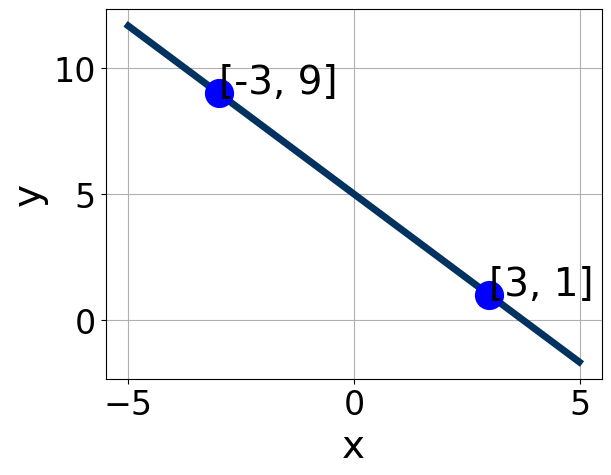
\includegraphics[width=0.5\textwidth]{../Figures/linearGraphToStandardB.png}
\end{center}
\begin{enumerate}[label=\Alph*.]
\item \( A \in [1.6, 5.3], \hspace{3mm} B \in [-3.06, -2.19], \text{ and } \hspace{3mm} C \in [-20, -12] \)
\item \( A \in [1.6, 5.3], \hspace{3mm} B \in [2.68, 3.08], \text{ and } \hspace{3mm} C \in [15, 18] \)
\item \( A \in [1.1, 3.6], \hspace{3mm} B \in [-1.07, -0.62], \text{ and } \hspace{3mm} C \in [-7, 0] \)
\item \( A \in [-9, -3], \hspace{3mm} B \in [-3.06, -2.19], \text{ and } \hspace{3mm} C \in [-20, -12] \)
\item \( A \in [1.1, 3.6], \hspace{3mm} B \in [0.83, 1.71], \text{ and } \hspace{3mm} C \in [1, 13] \)

\end{enumerate} }
\litem{
Solve the equation below. Then, choose the interval that contains the solution.\[ -9(-14x + 11) = -18(7x -6) \]\begin{enumerate}[label=\Alph*.]
\item \( x \in [0.03, 0.04] \)
\item \( x \in [-0.03, 0.01] \)
\item \( x \in [0.82, 0.83] \)
\item \( x \in [-0.07, -0.03] \)
\item \( \text{There are no real solutions.} \)

\end{enumerate} }
\litem{
Find the equation of the line described below. Write the linear equation in the form $ y=mx+b $ and choose the intervals that contain $m$ and $b$.\[ \text{Perpendicular to } 7 x - 4 y = 15 \text{ and passing through the point } (2, -5). \]\begin{enumerate}[label=\Alph*.]
\item \( m \in [0.08, 1.18] \hspace*{3mm} b \in [-6.79, -5.47] \)
\item \( m \in [-1.15, 0.33] \hspace*{3mm} b \in [-7.55, -6.33] \)
\item \( m \in [-1.15, 0.33] \hspace*{3mm} b \in [-4.77, -3.59] \)
\item \( m \in [-1.78, -1] \hspace*{3mm} b \in [-4.77, -3.59] \)
\item \( m \in [-1.15, 0.33] \hspace*{3mm} b \in [3.2, 4.62] \)

\end{enumerate} }
\litem{
Write the equation of the line in the graph below in Standard Form $Ax+By=C$. Then, choose the intervals that contain $A, B, \text{ and } C$.
\begin{center}
    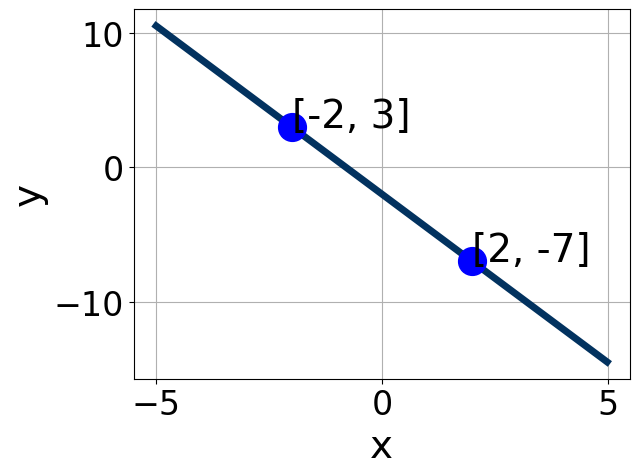
\includegraphics[width=0.5\textwidth]{../Figures/linearGraphToStandardCopyB.png}
\end{center}
\begin{enumerate}[label=\Alph*.]
\item \( A \in [0.4, 4.1], \hspace{3mm} B \in [0.95, 1.55], \text{ and } \hspace{3mm} C \in [-2.54, -1.9] \)
\item \( A \in [-7.1, -3.9], \hspace{3mm} B \in [-2.17, -1.4], \text{ and } \hspace{3mm} C \in [3.28, 4.82] \)
\item \( A \in [4.8, 7.2], \hspace{3mm} B \in [1.19, 2.03], \text{ and } \hspace{3mm} C \in [-5.16, -3.1] \)
\item \( A \in [4.8, 7.2], \hspace{3mm} B \in [-2.17, -1.4], \text{ and } \hspace{3mm} C \in [3.28, 4.82] \)
\item \( A \in [0.4, 4.1], \hspace{3mm} B \in [-1.28, -0.62], \text{ and } \hspace{3mm} C \in [0.68, 2.36] \)

\end{enumerate} }
\litem{
Find the equation of the line described below. Write the linear equation in the form $ y=mx+b $ and choose the intervals that contain $m$ and $b$.\[ \text{Perpendicular to } 5 x + 4 y = 13 \text{ and passing through the point } (4, 7). \]\begin{enumerate}[label=\Alph*.]
\item \( m \in [0.68, 1.24] \hspace*{3mm} b \in [-3.86, -3.23] \)
\item \( m \in [0.68, 1.24] \hspace*{3mm} b \in [3.48, 4.1] \)
\item \( m \in [-1.73, -0.68] \hspace*{3mm} b \in [10.01, 10.27] \)
\item \( m \in [0.82, 1.33] \hspace*{3mm} b \in [3.48, 4.1] \)
\item \( m \in [0.68, 1.24] \hspace*{3mm} b \in [2.56, 3.07] \)

\end{enumerate} }
\litem{
Solve the equation below. Then, choose the interval that contains the solution.\[ -14(-5x -19) = -18(-13x -11) \]\begin{enumerate}[label=\Alph*.]
\item \( x \in [0.1, 0.7] \)
\item \( x \in [-2.5, -0.8] \)
\item \( x \in [1.9, 3] \)
\item \( x \in [-3.4, -2] \)
\item \( \text{There are no real solutions.} \)

\end{enumerate} }
\litem{
First, find the equation of the line containing the two points below. Then, write the equation in the form $ y=mx+b $ and choose the intervals that contain $m$ and $b$.\[ (-2, 11) \text{ and } (-7, -2) \]\begin{enumerate}[label=\Alph*.]
\item \( m \in [1.6, 11.6] \hspace*{3mm} b \in [12.6, 15.6] \)
\item \( m \in [-4.6, 0.4] \hspace*{3mm} b \in [-23.9, -16.6] \)
\item \( m \in [1.6, 11.6] \hspace*{3mm} b \in [-16.3, -16.1] \)
\item \( m \in [1.6, 11.6] \hspace*{3mm} b \in [15, 18.1] \)
\item \( m \in [1.6, 11.6] \hspace*{3mm} b \in [3.5, 6] \)

\end{enumerate} }
\litem{
Solve the linear equation below. Then, choose the interval that contains the solution.\[ \frac{3x -4}{8} - \frac{-8x + 5}{3} = \frac{8x + 7}{5} \]\begin{enumerate}[label=\Alph*.]
\item \( x \in [1.8, 5.3] \)
\item \( x \in [-1.2, 0.6] \)
\item \( x \in [0.6, 2] \)
\item \( x \in [9.2, 12.7] \)
\item \( \text{There are no real solutions.} \)

\end{enumerate} }
\end{enumerate}

\end{document}